\begin{figure}[t!]
  \centering
  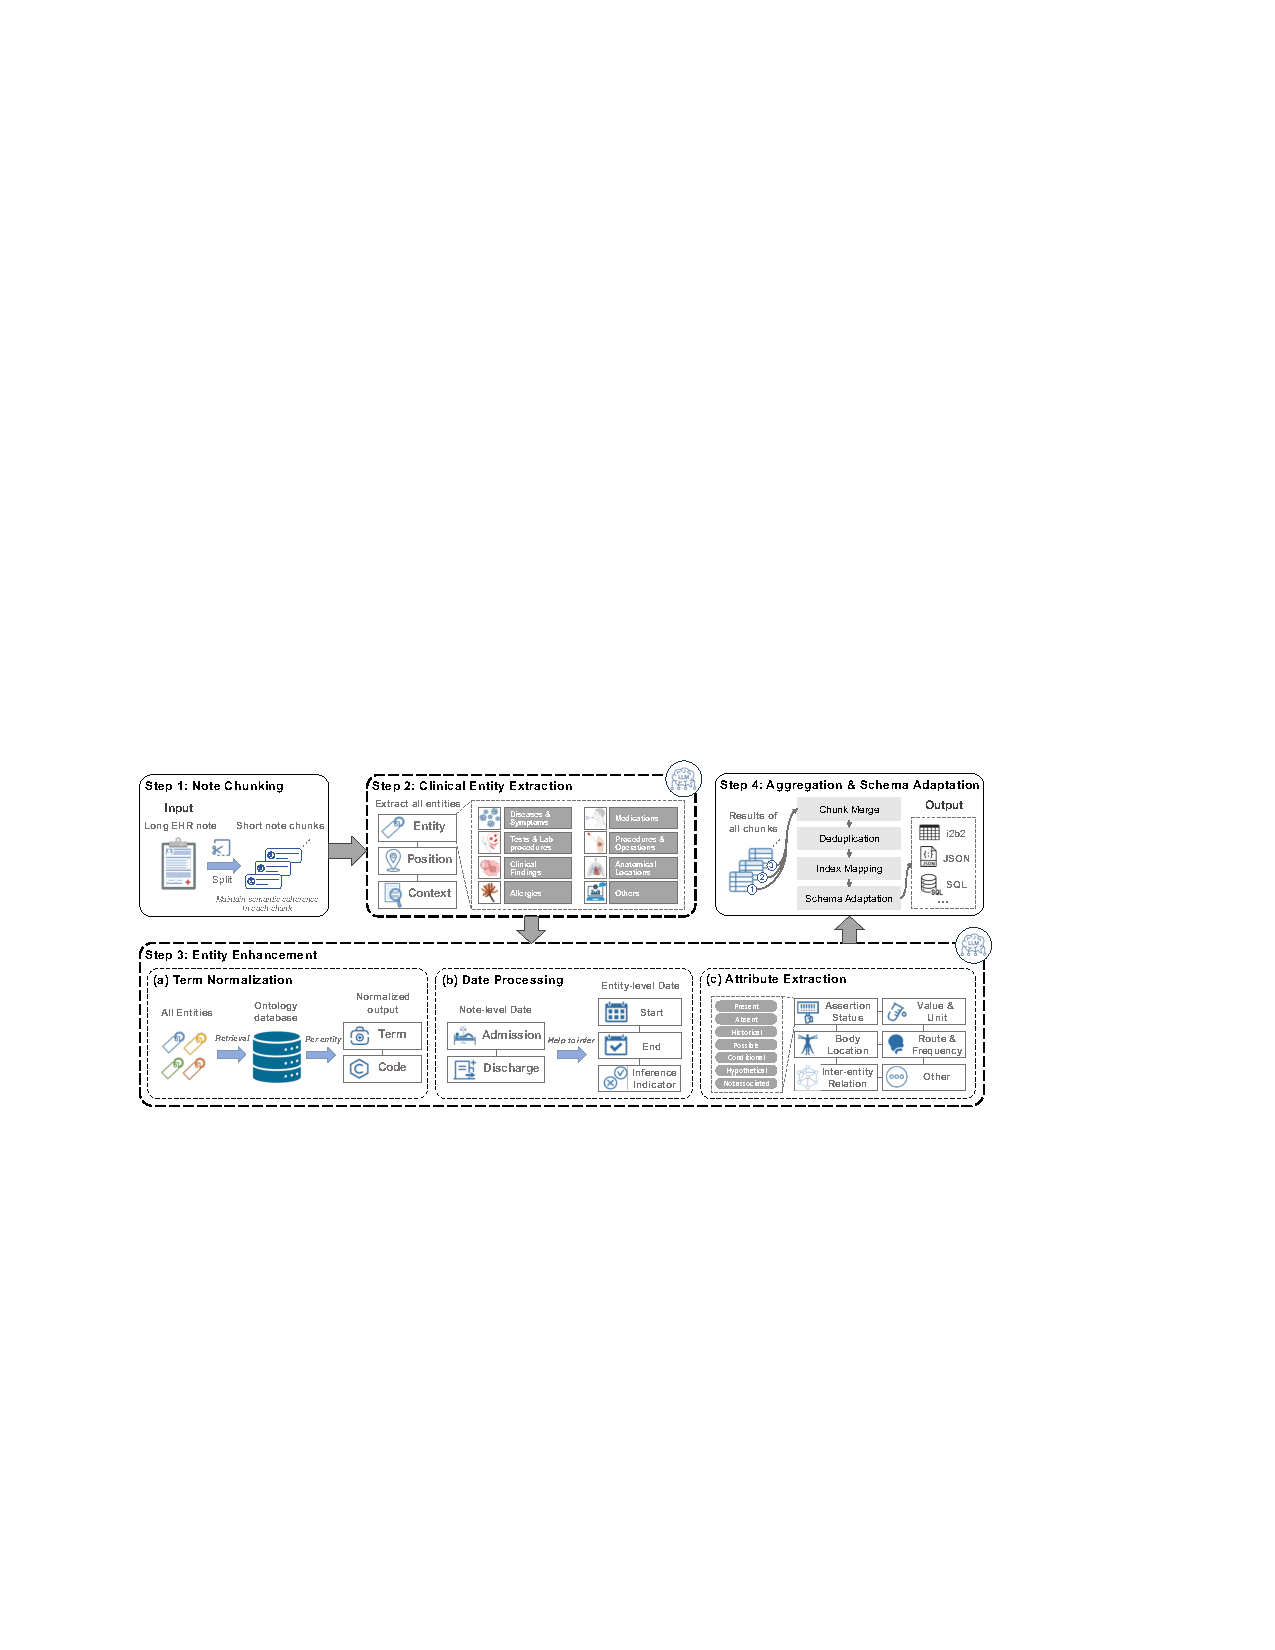
\includegraphics[width=\linewidth,height=0.9\textheight,keepaspectratio]{figures/figure1.pdf}\vspace{-9mm}
  \caption{\textbf{Overview of CLINES.} Step 1, segments long clinical notes into semantically coherent chunks to constrain LLM's context window and improve robustness. Step 2, from each chunk, extract clinical entities with broad coverage, including medications, diseases, and laboratory tests. Step 3, for each entity, uses local context to: (a) normalize to an ontology term with a unique code; (b) for event-type entities, extract or infer start and end dates, when imprecise; and (c) infer assertion status and capture clinically relevant modifiers, e.g., for medications: dose, unit, frequency, and route; for tests: numeric values (with units); for diseases: activity status and other pertinent attributes. Step 4, reconciles entity-level information across all chunks and exports results in user-specified formats (e.g., i2b2, JSON, SQL).}
  \label{fig:clines-overview}
\end{figure}
